\section{Introduction}
Humans are considered a social creature.
Almost everyone has interaction with other people and this shapes our language.
But not everyone speaks the same language.
Different countries have different language, even some countries have multiple languages.
Regions can have different and even multiple dialects.
Humans are limited in the number of interactions they can have, which can create a constraint on the evolution of language.

This paper is a variation on the work done by \cite{de2010multi} and uses this as a starting point in which social dynamics will be taken into account.
The original work uses an \textit{Intimidation game} to see how combinatorial phonology can spread.
Their approach was an agent-based system where every agent was equipped with four trajectories.
A trajectory is a combinatorial structure that can be seen as an utterance of a word.
Trajectories are, however, an abstraction over this.
\citeauthor{de2010multi} have as goal to look at the emergence of distinct clusters that optimize acoustics distinction.
If words have different sounds, it makes it easier to understand each other.

\begin{figure}[t]
    \centering
    \begin{subfigure}[t]{0.3\textwidth}
        \centering
        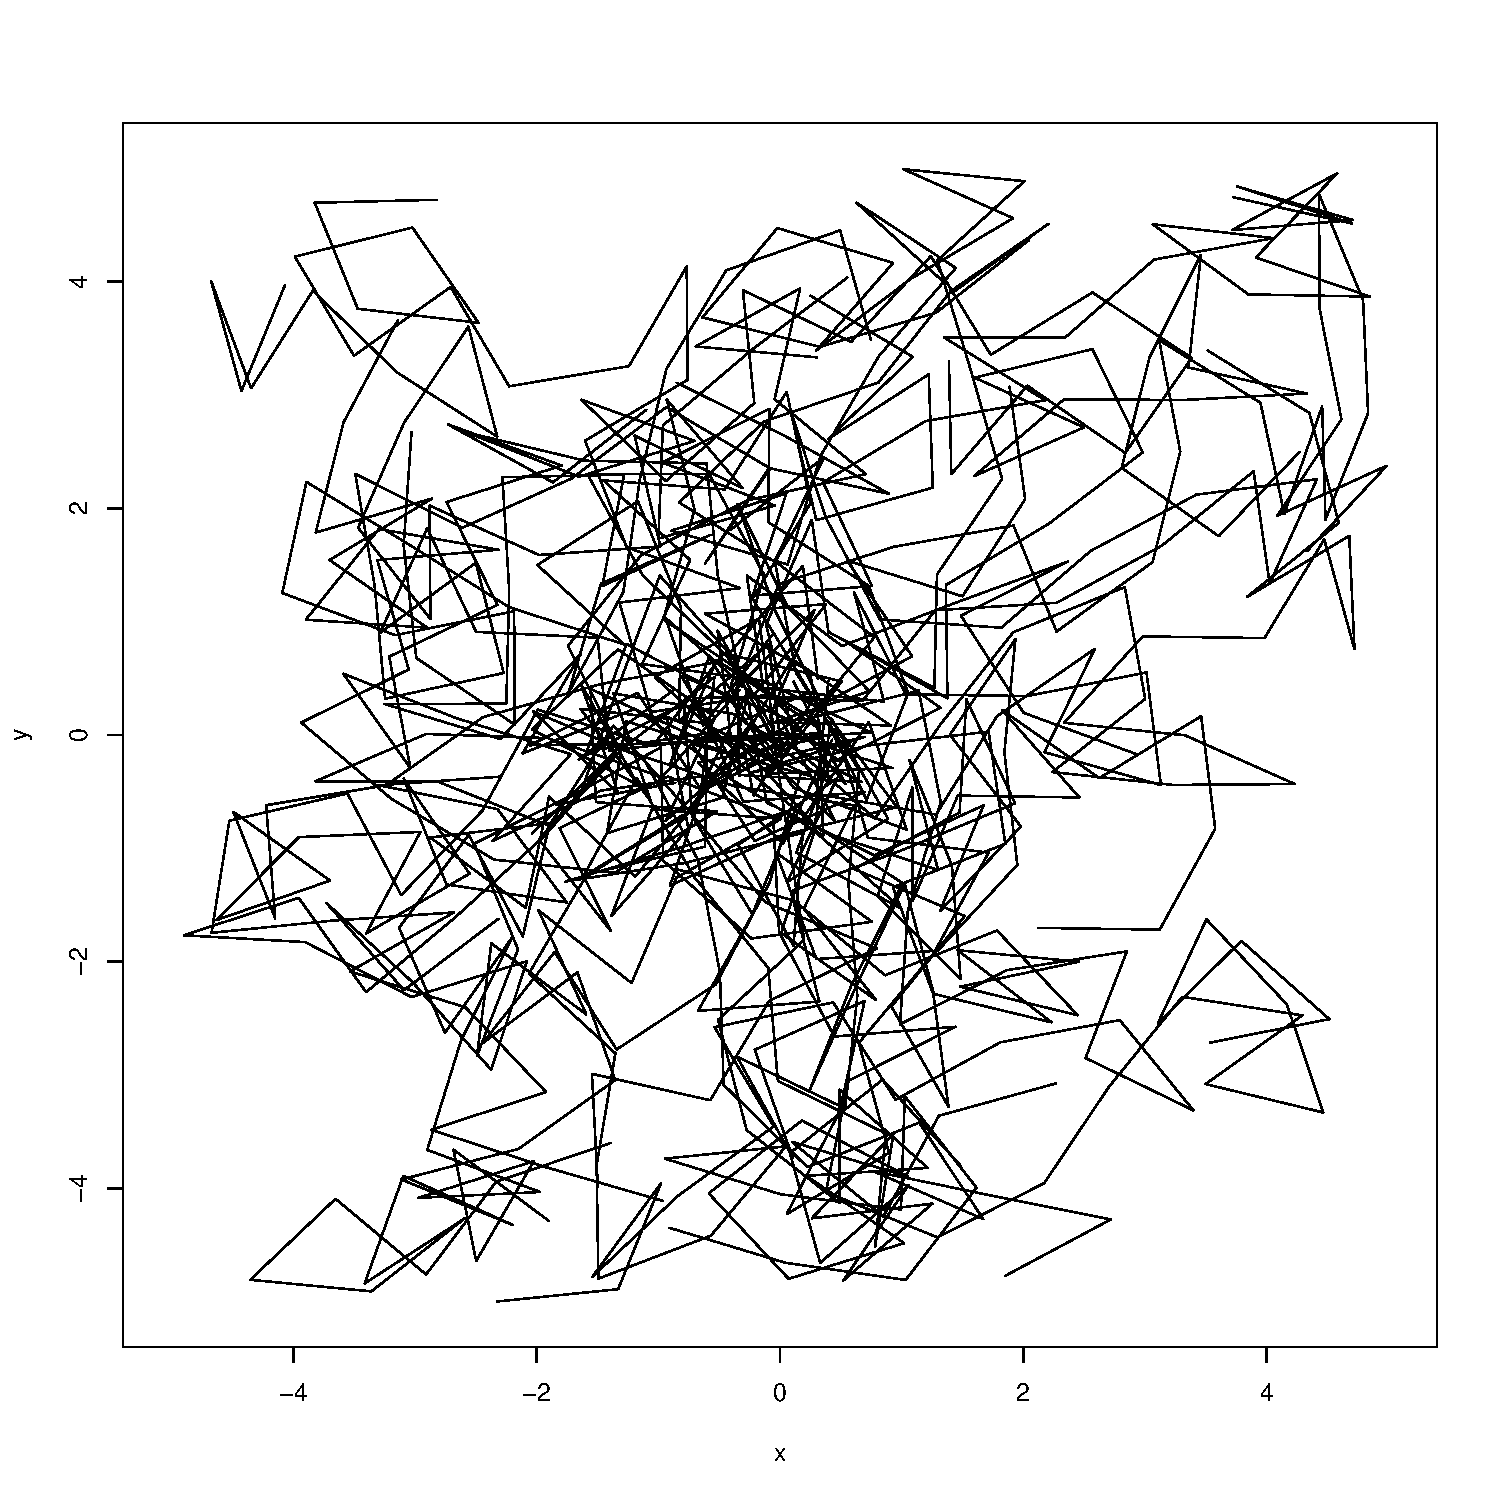
\includegraphics[width=\textwidth]{Traject4Init.pdf}
        \caption{The trajectories of ten agents before the simulation begins.}
        \label{fig:Traject4Init}
    \end{subfigure}
    \hfill
    \begin{subfigure}[t]{0.3\textwidth}
        \centering
        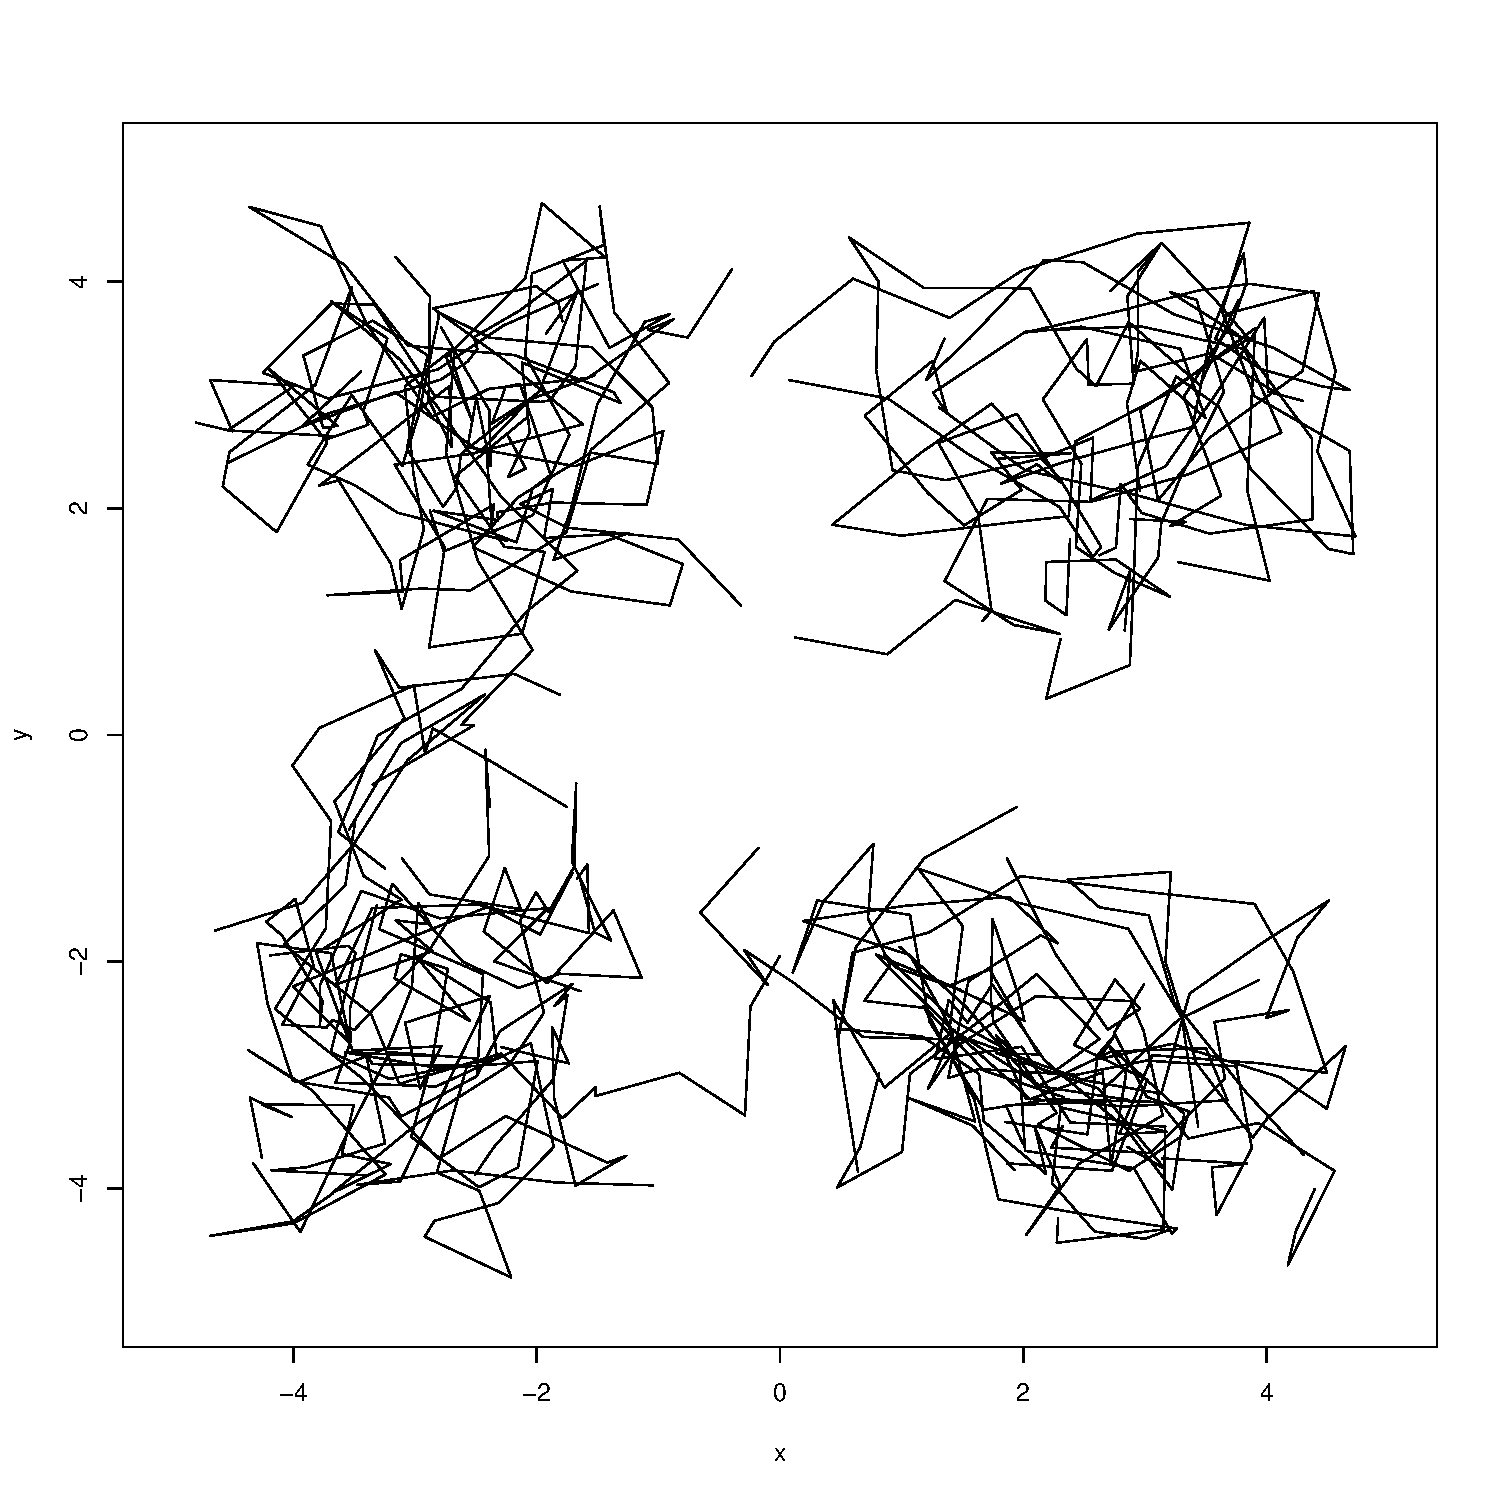
\includegraphics[width=\textwidth]{Traject4Res.pdf}
        \caption{The resulting trajectories of the ten agents after the simulation.}
        \label{fig:Traject4Res}
    \end{subfigure}
    \hfill
    \begin{subfigure}[t]{0.3\textwidth}
        \centering
        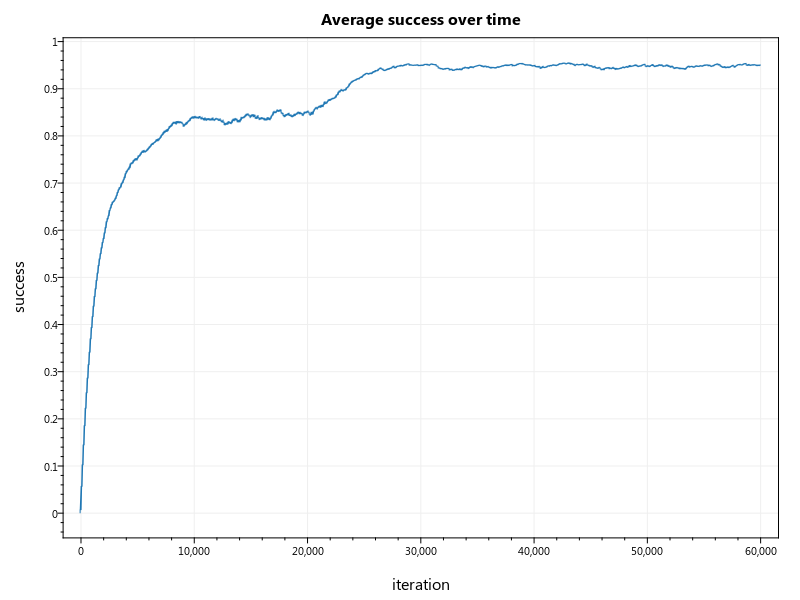
\includegraphics[width=\textwidth]{Traject4Success.png}
        \caption{The running average success of the simulation.}
        \label{fig:Traject4Success}
    \end{subfigure}

    \caption{System of trajectories \autoref{fig:Traject4Init} before and \autoref{fig:Traject4Res} after 60.000 iterations. \autoref{fig:Traject4Res} shows four clusters, each containing one trajectory of each agent.}
    \label{fig:Traject4}
\end{figure}

The results are very promising and shows that with a population of 10 agents and four trajectories, the trajectories are driven to the corners.
This indicates the emergence of the distinct clusters.
A replication of this result can be found in \autoref{fig:Traject4}.
\autoref{fig:Traject4Init} shows the trajectories before the simulation starts and \autoref{fig:Traject4Res} shows the resulting clusters.
These are similar result to what is found in the work of \cite{de2010multi}.

One of the reasons this result differs somewhat from the original work, is a mistake in the original paper.
The original paper says:
\begin{quotation}
    $\dots$, the agent plays repeated imitation games with \textbf{all} other agents in the population (called \textit{imitators}). 
\end{quotation}
while the pseudo-code in this paper says:

\begin{algorithm}
    \caption{DISTRIBUTED OPTIMIZATION(A)}
    \begin{algorithmic}

        % \mbox{other code}
        % \Comment{e}
        \State $\dots$
        \State 

        \Loop $N_{test}$ \textbf{times}

            \State $imitator$ $\leftarrow$ random agent from $A$, different from $initiator$

            \State $\dots$
        \EndLoop

        \State
        \State $\dots$
        
    \end{algorithmic}
\end{algorithm}

(note that this is a snipped of the pseudo-code found in \citep*{de2010multi}).

It is clear that this might be a small mistake but it has a great impact on how the simulation plays out.

To clear things up, the method chosen for this paper is more inline with what was said in the original paper and not the pseudo-code.
The difference of this change on the original work and this paper are interesting to test and may be needed to validate some of the results down the line.

